\chapter{Appraisal}
	
	\section{Comparison of project performance against numbered general
and specific objectives}

My objectives from Section 1 were:

\begin{enumerate}
			\item{Have a main menu that allows the user to
select different options.}

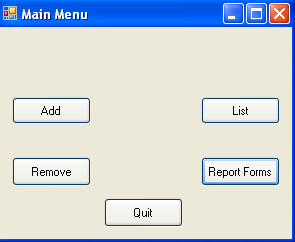
\includegraphics[scale=0.5]{frmMainMenu_scrot}
			\item{Have a functioning relational database,
queriable with SQL, made in Microsoft Access, with the required number of
tables.}

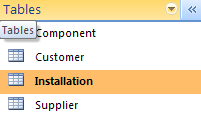
\includegraphics[scale=0.5]{dbtablesscrot_scrot}
			\item{Enable the user to add customers.}
			
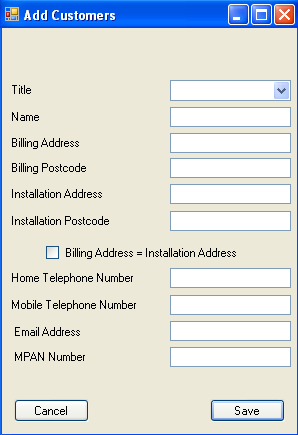
\includegraphics[scale=0.5]{frmAddCustomer_scrot}
			\item{Enable the user to add suppliers.}
			
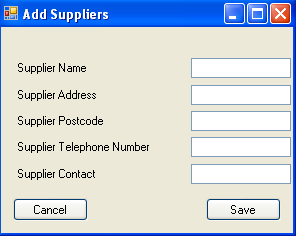
\includegraphics[scale=0.5]{frmAddSupplier_scrot}
			\item{Enable the user to add components.}
			
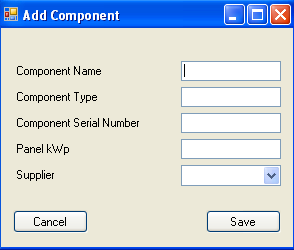
\includegraphics[scale=0.5]{frmAddComponent_scrot}
			\item{Enable the user to remove customers.}
			
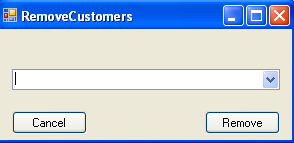
\includegraphics[scale=0.5]{frmRemoveCustomer_scrot}
			\item{Enable the user to remove suppliers.}

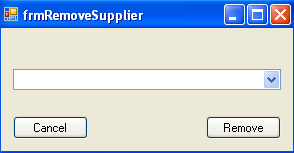
\includegraphics[scale=0.5]{frmRemoveSupplier_scrot}
			\item{Enable the user to remove components.}

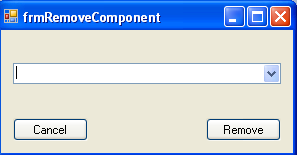
\includegraphics[scale=0.5]{frmRemoveComponent_scrot}
			\item{Enable the user to list customers.}
			
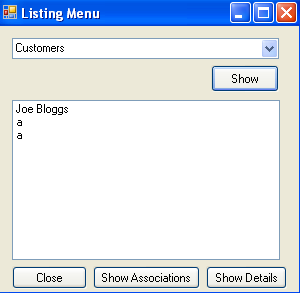
\includegraphics[scale=0.5]{frmList_cust_scrot}
			\item{Enable the user to list suppliers.}
			
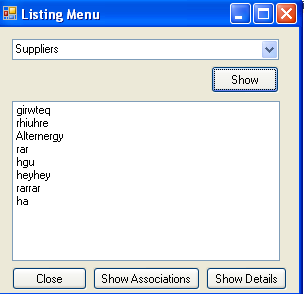
\includegraphics[scale=0.5]{supplier-frmList-second_scrot}
			\item{Enable the user to list components.}
			
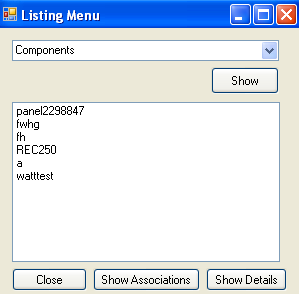
\includegraphics[scale=0.5]{frmList_comp_scrot}
			\item{Enable the user to view and edit invoices, log forms,
and reports in Microsoft Word by clicking buttons in the program to open
the requested forms.}

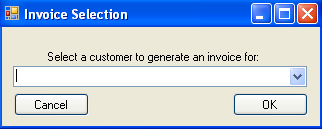
\includegraphics[scale=0.5]{invoice_menu_scrot}
			\item{Enable the user to view relationships between
suppliers and the components they stock.}

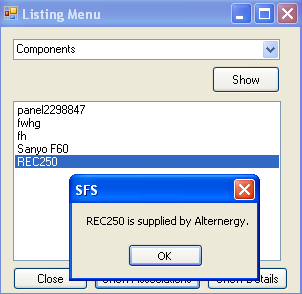
\includegraphics[scale=0.5]{component-frmList-sa_scrot}
			\item{The program must input data into the invoices
and quotes to avoid the user having to duplicate data entry, and this data
must come from either user input or data from the database.}
			\begin{itemize}
				\item{Objective fourteen is partially acheived due to the invoices being populated
				with the chosen customer's address, and a header `INVOICE'.}
			\end{itemize}
			

\includegraphics[scale=0.5]{invoice_info_now_scrot}
			\item{The system should be menu-driven, with
consistent GUI form layout throughout, as far as possible.}
			\begin{itemize}
				\item{See all of the forms for evidence of this: they are menus.}
			\end{itemize}
			\item{Enable printing directly from the program for
the user to print lists of customers etc.}
			\begin{itemize}
				\item{This has not been acheived due to the unexpected complexity of
				printing to an actual printer in VB.NET.  Luckily, this objective was not strictly
				necessary due to the reports being able to be printed via Microsoft Word
				when they opened.}
			\end{itemize}
			\item{Enable searching of customers, suppliers and components, and sort the search results.}
			\begin{itemize}
				\item{This objective is partially achieved: the sorting of the search results was not implemented due to time constraints.}
			\end{itemize}
			
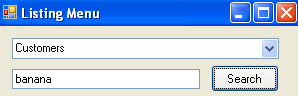
\includegraphics[scale=0.5]{searching_demo_scrot1}
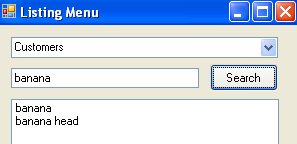
\includegraphics[scale=0.5]{searching_demo_scrot2}
\end{enumerate}

I have acheived objectives one, two, three, four, five, six, seven, eight,
nine, ten, eleven, twelve, thirteen and fifteen in full.  These objectives are referenced clearly in the code comments, with screenshots above in the bulleted list.

	\section{User feedback authenticated by the assessor}
	
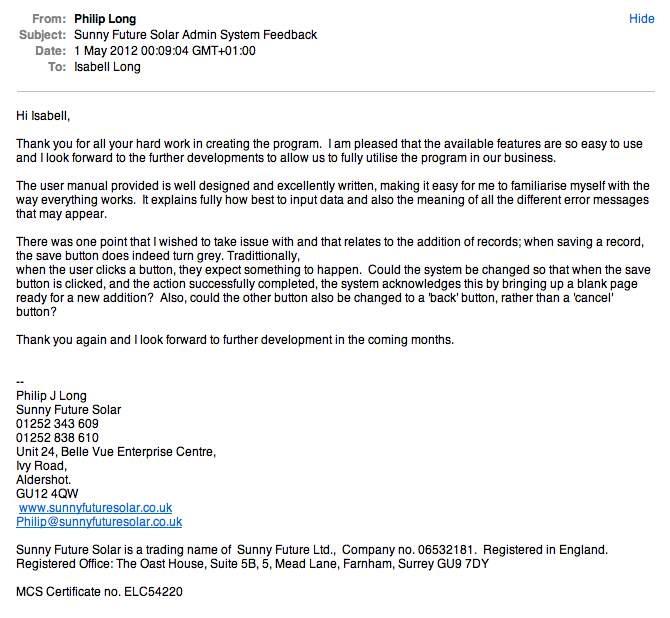
\includegraphics[scale=0.65]{user_feedback_scrot}
	
	\section{Analysis of user feedback}
	
\begin{itemize}
	\item{Philip liked the user manual and its layout and the explanation of error messages.}\\
	\item{He ``looked forward to further developments'', of which there are a few that he picked up on:}\\
	\begin{itemize}
		\item{The user interface needs some work with regard to the add customer\slash supplier\slash component forms, with it at present not telling the user when a customer etc. has been successfully inserted and not leading them back to the form to enter another customer.  Philip's suggestion is possible to implement with a loop: if there are no errors then insert into the database and, if successful, loop back around to the empty `Add[Customer|Supplier|Component] form for ease of data entry.}\\
		\item{Also UI related, Philip requested that the Cancel button on each of the addition forms be changed to a Close button, because then it does not give the impression that the user is eradicating a legitimate change, or has made one even when the form is blank.  This is possible through simply changing a few procedure and variable names and references.}\\
	\end{itemize}
\end{itemize}
	\section{Possible extensions}

Lots could be done to extend the feature set of this project, including fixes for the issues raised in the user feedback, and:

\begin{itemize}
	\item{Displaying invoices and quotations within the program itself, using a report viewer integrated into VB, not having to go through Microsoft Word, enabling the information to be displayed more quickly and reducing the amount of times the user has to click.}
	\item{Enabling printing of the aforementioned invoices and
quotations from within VB.  This would be faster as the computer would not have to load a word processor and the user would not have to click three buttons---only one.}
	\item{Enabling the invoices and quotations to display everything
they should display: the selected components going to be installed and installation price to name but a few things.}
	\item{Finishing development of the survey form.}
	\item{Rewriting the program as a console application in Ruby as another
learning experience?  This would make the program cross-platform and---with the absence of buttons and graphics---potentially more simple.}
\end{itemize}
